\subsection{Classical Beauty Contest}

The classical Beauty Contest game\footnote{Also widely referred to as Guess 2/3 of the average \citep{ledoux1981concours}, p-contest \citep{kennerberg2019convergence}, and p-guessing game \citep{vie2021evolutionary}} can be mathematically formulated as a set of $N$ players, each of them choosing an integer number in some interval, often from 0 to 100. The mean value $\bar{n}$ of these $N$ numbers is then calculated and, given a certain positive constant $p$, which is generally known by all players before the game, the winning number of the contest is given by $w=p\,\bar{n}$ (rounded to the closest integer in the range). The value $p$, which is commonly taken to be $1/2$ or $2/3$, determines a shift of the winning number from the mean guess, and therefore represents the motivation for a certain level of recursive reasoning in the player's choice, analogous to the original Beauty Contest formulation.\\

As an example of a contractive Beauty Contest with factor $p=2/3$, in the first histogram in Fig. \ref{fig:1} we can see that a common strategy is to choose numbers close to the value $50\cdot p^k$ for some positive integer $k$ (i.e. 33, 22, ...). This indicates the different levels of recursion in the decision process, where one starts with the assumption that everybody will play a random number, producing most likely $\bar{n}=50$, and hence playing a value $50\cdot p\simeq 33$. The successive step is to think that everybody most likely will play $33$, hence the guess is  $33\cdot p=22$. This line of reasoning is called the $k$-level thinking model, where a player tries to outsmart the other players by playing one level ahead of them. This model predicts the agents to learn about their respective environment in successively played games, and in fact seems to predict the popular guesses fairly well, at least for small values of $k$.\\

One other popular guess in this iteration of the Beauty Contest seems to be 0, which is basically the limit of this $k$-level model when $k\to\infty$. In fact the scenario where every player guesses 0 is the unique Nash equilibrium for the Beauty Contest game (given $0< p<1$) \citep{kennerberg2019convergence}. However, in this case the assumption of perfect rationality of the other players is a strong one, and it is very naive to imagine that all the people will take this $k$-level model to the extreme consequences, thus practically invalidating the strategy of playing 0.\\

As expected, in this first iteration of the Beauty Contest with $p=2/3$, the winning number is not $w=0$, but rather $w=20$. If one then re-proposes the same game to the same group of $N$ people, the consequence is visible: people seem to adapt to the game environment and play on average much lower numbers, see the last two histograms in Fig. \ref{fig:1}.\\

It's now time to go quantum!

\begin{figure}[h]
    \centering
    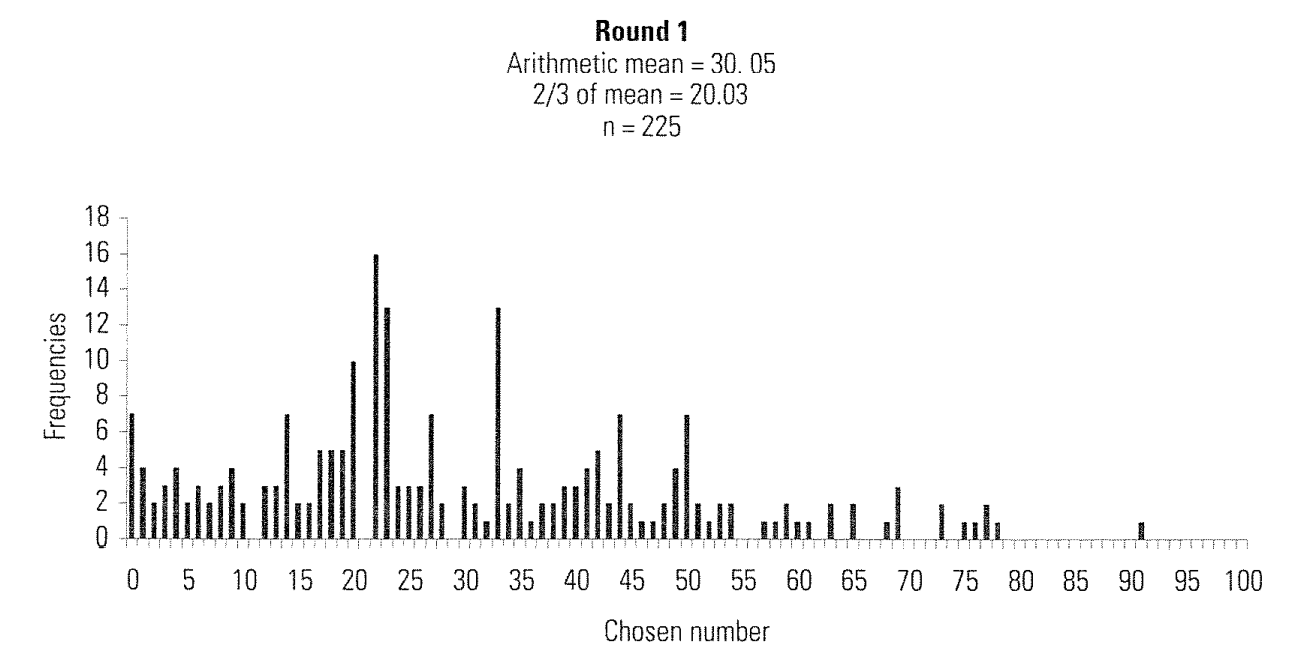
\includegraphics[width=0.45\textwidth]{chil-template-2023/images/round1_classical.png}\vspace{0.5cm}
    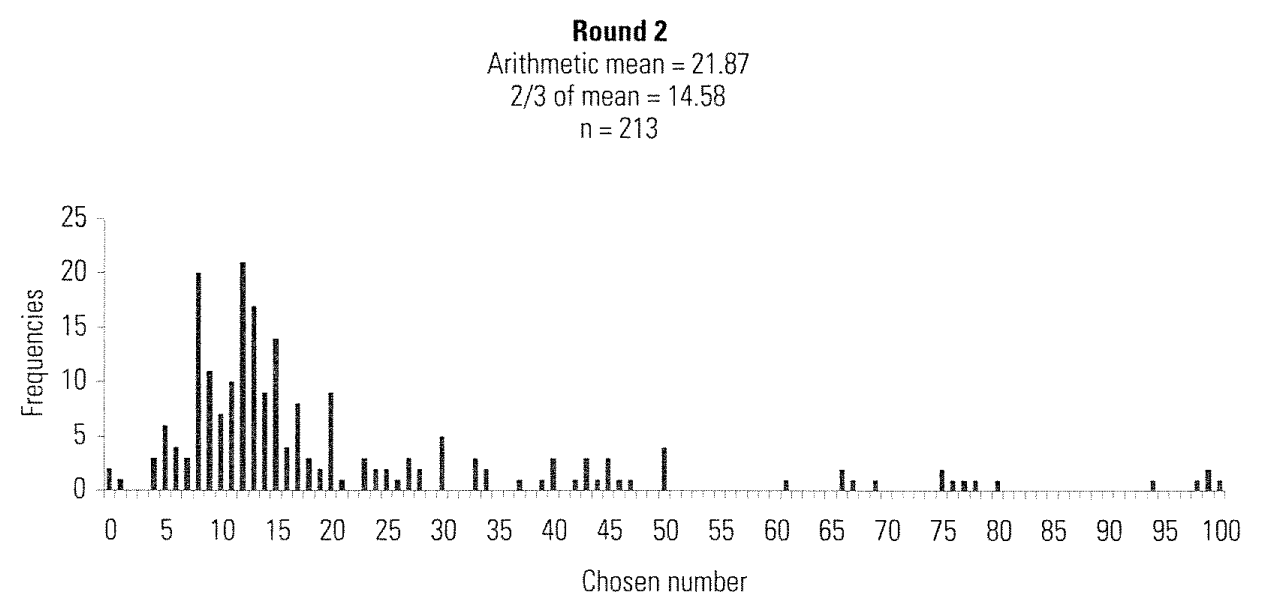
\includegraphics[width=0.45\textwidth]{chil-template-2023/images/round2_classical.png}\vspace{0.5cm}
    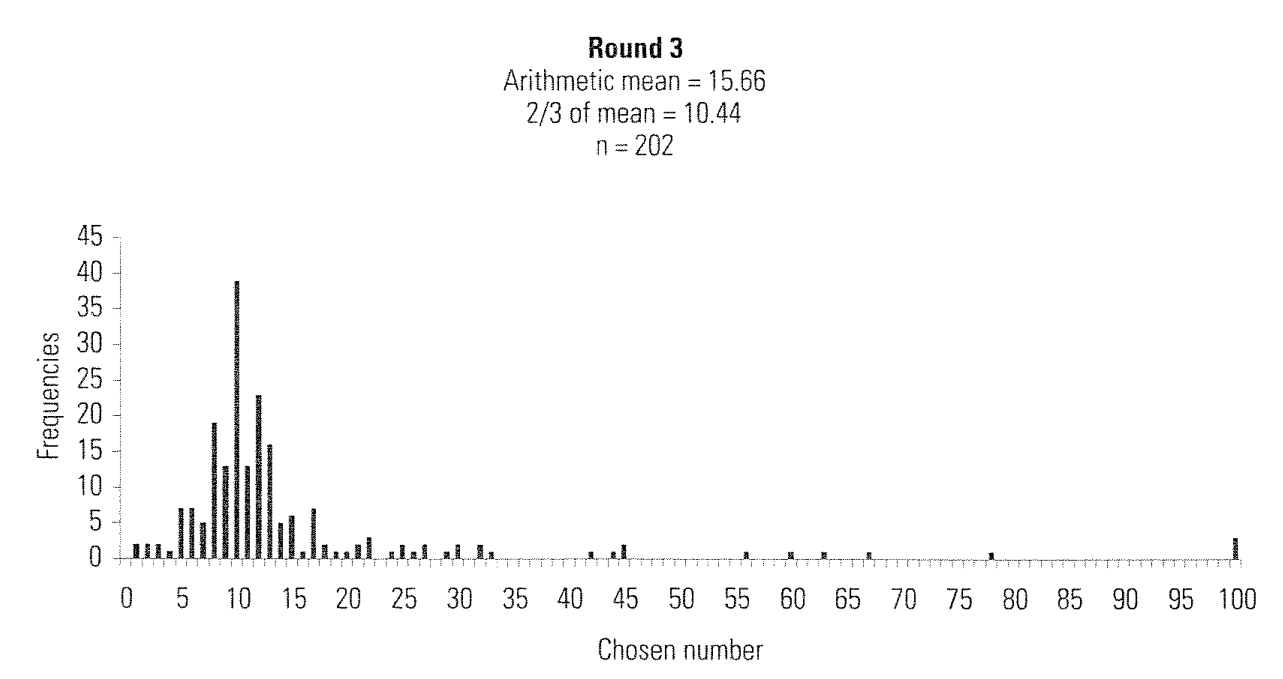
\includegraphics[width=0.45\textwidth]{chil-template-2023/images/round3_classical.png}
    \caption{From top to bottom: the first three rounds of the classical Beauty Contest results, with a value of $p=2/3$ \citep{diekmann2009classical}.}
    \label{fig:1}
\end{figure}

% \begin{figure*}
%   \centering
%   \captionsetup{width=0.8\textwidth}
%   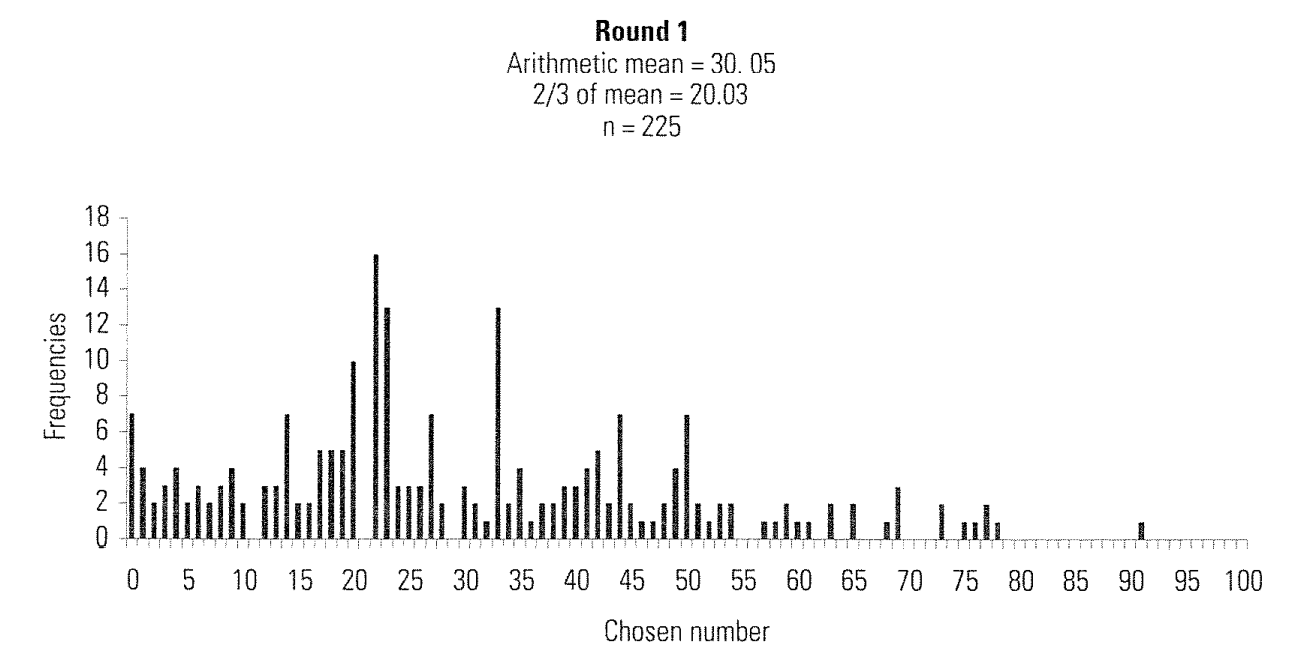
\includegraphics[width=0.8\textwidth]{chil-template-2023/images/round1_classical.png}\vspace{0.5cm}
%   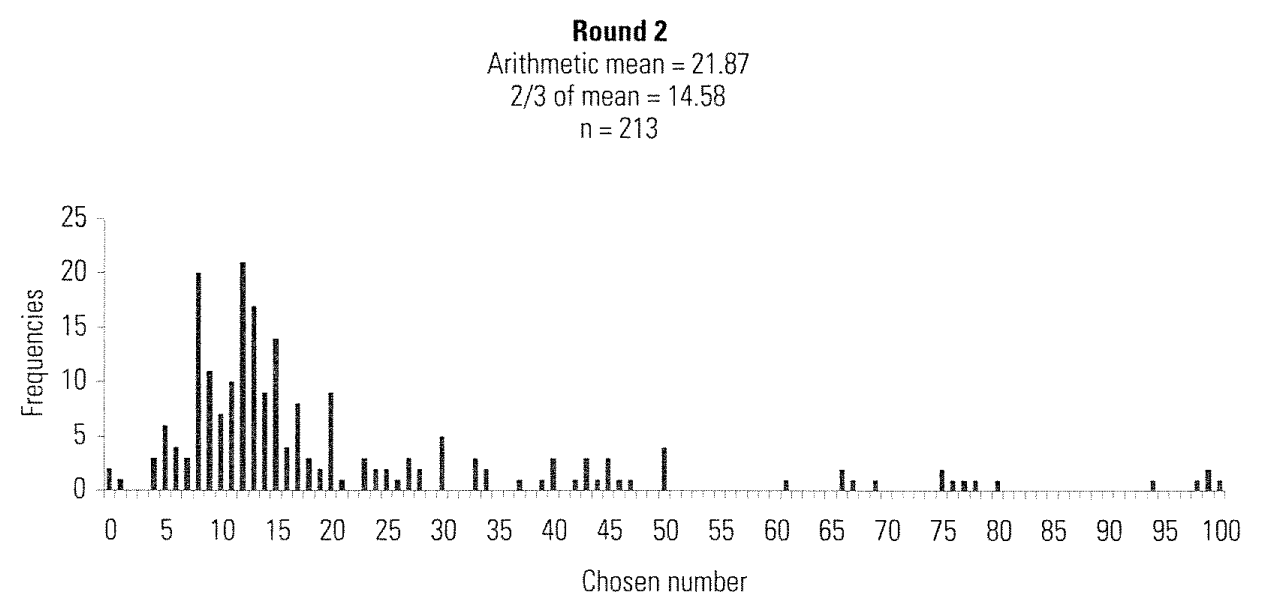
\includegraphics[width=0.8\textwidth]{chil-template-2023/images/round2_classical.png}\vspace{0.5cm}
%   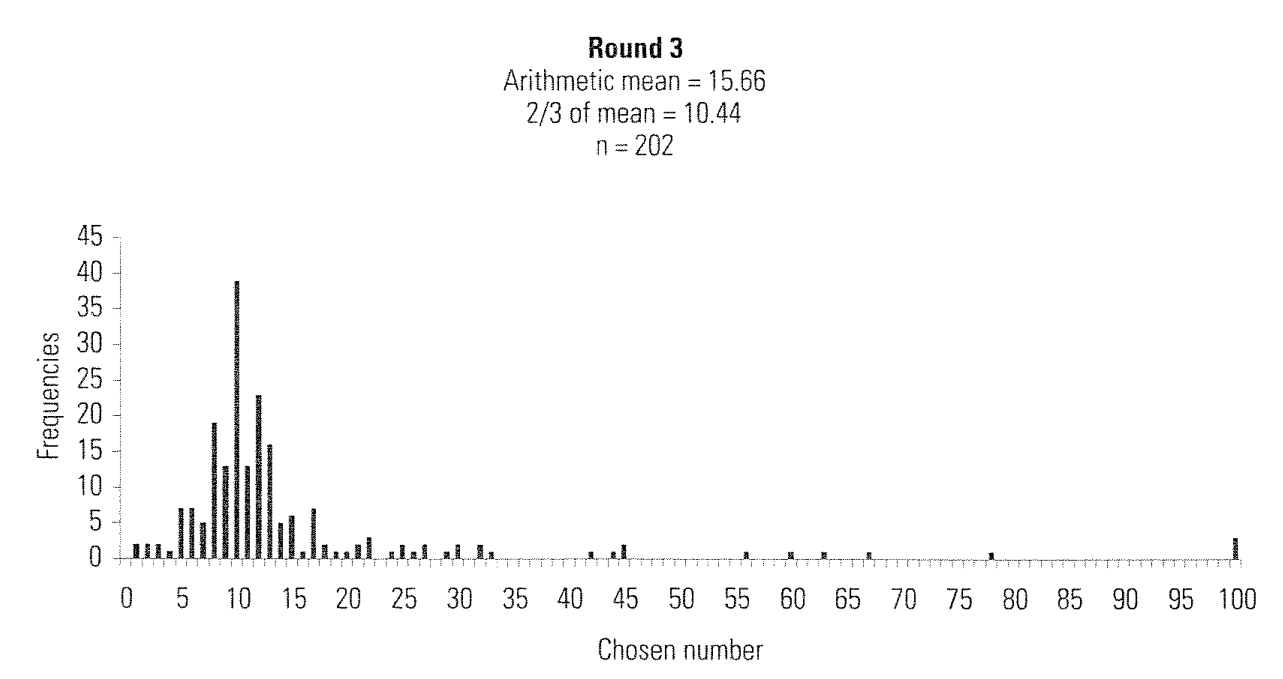
\includegraphics[width=0.8\textwidth]{chil-template-2023/images/round3_classical.png}
%   \caption{From top to bottom: the first three rounds of the classical Beauty Contest results, with a value of $p=2/3$ \citep{diekmann2009classical}.}
%   \label{fig:1}
% \end{figure*}

\subsection{Quantum Beauty Contest}

The game we are considering again takes $N$ players, each of one will formulate a guess. In this scenario however, the guess is formulated in terms of quantum states. For this, we construct a $(M+1)$ dimensional Hilbert space $\mathcal{H}_M$, where for concreteness we will choose $M=100$. This space is spanned by the following base kets, in standard Dirac notation:
\begin{equation}
  \label{eq:basis}
  \Bigl\{\ket{0},\ \ket{1},\ \ket{2},\,...\,\ket{100}\Bigr\}
\end{equation}

which are the eigenstates of a number operator $\hat{N}$ with explicit form 
\begin{equation}
    \hat{N} = \sum_{n=0}^{100} n \ket{n}\bra{n}
\end{equation}

from which we can immediatly see the defining property
\begin{equation}
    \label{eq:number_operator}
    \hat{N}\ket{n} = n \ket{n}.
\end{equation}

Furthermore, the basis is generally chosen to be normalized:
\begin{equation}
    \label{eq:normalization}
    \braket{n|m} = \delta_{nm}
\end{equation}

where $\delta_{nm}$ is the Kronecker delta.\\

In a certain sense, the base kets represent the guesses a player can make in the classical game. Now, in this variation of the game, each player is asked to give a guess in the form of a normalized ket:
\begin{equation}
  \ket{\psi_i}\in\mathcal{H}_M \quad \text{for}\quad  i\in\{1,2,\,...\,N\},
\end{equation}

i.e.
\begin{equation}
    \ket{\psi_i} = \sum_{n=0}^{100} c_n^{(i)} \ket{n}\quad \text{and}\quad \sum_{n=0}^{100} \, |c_n^{(i)}|^2 = 1\quad \forall i.
\end{equation}

Then the following ket state is constructed:
\begin{equation}
\label{eq:game_ket}
  \ket{\psi}=\mathcal{N}\,\sum_{i=1}^{N}\ket{\psi_i}
\end{equation}

where $\mathcal{N}$ is some normalization constant.\\

The following step is to collapse our state $\ket{\psi}$ into the basis given in Eq. \ref{eq:basis}, that is to say, we perform a measurement of $\hat{N}$ on $\ket{\psi}$.\\

We will therefore obtain as a state the ket
\begin{equation}
  \ket{n},\quad \text{with }n\in\{0,1,\,...\,100\}
\end{equation}

with a probability
\begin{equation}
  P_n=|\braket{n|\psi}|^2.
\end{equation}

The winning number is then determined as usual as
\begin{equation}
  w=\text{round}(p\cdot n)
\end{equation}

for some positive $p$. With this number, we can single out the basis ket $\ket{w}$ and determine the winner(s) of the Quantum Beauty Contest by assigning a payoff to each player via the following formula:
\begin{equation}
  \phi_i=|\braket{w|\psi_i}|^2
\end{equation}

which is basically a simple measure for telling how much of the winning outcome was contained in the player's initial guess.\\

From a theoretical point of view, the Quantum Beauty Contest we propose does not reduce to its classical analogue for any choice of the players' strategies. This is due to two independent features of the quantum version of the game.\\

Firstly, the winning number $w$ is produced through a measurement procedure of the state $\ket{\psi}$, hence there is a component of randomness in this game which is not present in the classical version.\\

Secondly, even if one repeated the measurement of the same state $\ket{\psi}$ over and over again, thus effectively
extracting the mean value of the operator $\hat{N}$ (which will be in fact done in some later computational implementations of the game), in general there is no strategy of the players that can simulate the classical analogue of the game. This is because the way we decided to construct the state $\ket{\psi}$ is through the sum with equal weights of the guesses $\ket{\psi_i}$. In this game, the only strategy that resembles a classical game is for every player to play a ket in the basis of Eq. \ref{eq:basis}:
\begin{equation}
  \ket{\psi_i}=\ket{n},\quad \text{for some }n\in\{0,1,\,...\,100\}
\end{equation}

In this way though, if two players decide to play the same number, i.e. $\ket{\psi_i}=\ket{\psi_j}=\ket{n}$ with $i\neq j$, then the probability amplitudes in the state $\ket{\psi}$ for the basis state $\ket{n}$ add up, while the actual probability of extracting the number $n$ goes as the amplitude squared. This is in contrast with the classical game, where every instance of a guess $n$ simply adds up and the mean is calculated afterwards without squaring the columns of the histogram.\\

Anyway, apart from these differences, the spirit of the game remains the same, but in this case the strategy space is much richer than the classical counterpart.\\





% (NASH EQUILIBRIUM CLASSICAL)

% (CITE PAPERS)

% (LEVEL k-MODEL)

% (AGENTS ARE LEARNING ABOUT THEIR RESPECTIVE ENVIRONMENT)